\documentclass[aspectratio=169]{beamer}
\usetheme{metropolis}
\usepackage{graphics}
\usepackage{longtable}
\usepackage{scrextend}

\title{CPS - Projet - Loderunner}
\date{\today}
\author{Basile Pesin, David Sreng}
\institute{Faculté des Sciences de Sorbonne Université}

\begin{document}
\maketitle

\begin{frame}
  \begin{center}
    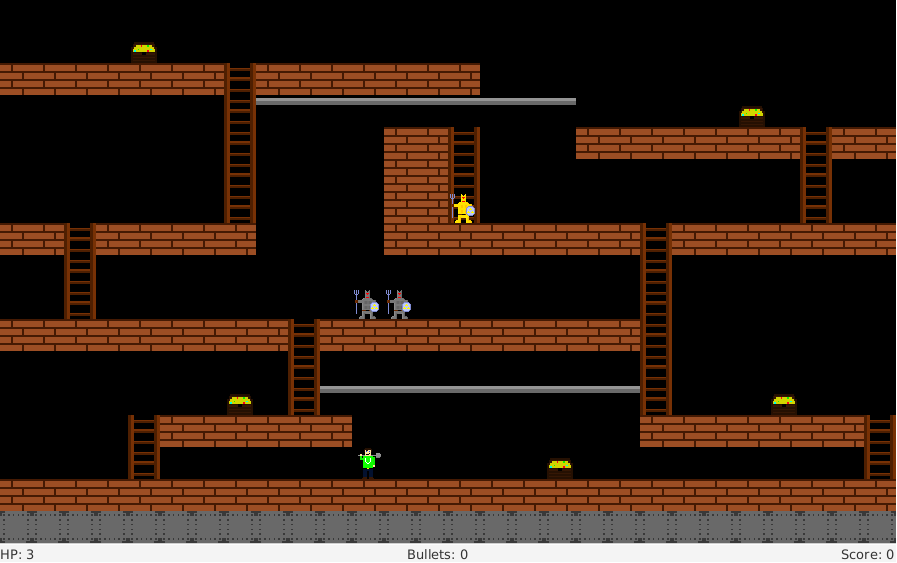
\includegraphics[height=0.7\paperheight]{assets/game.png}
  \end{center}
\end{frame}

\begin{frame}{Extensions}
  \begin{itemize}
    \item Amélioration de l'IA des gardes
    \item Armes à feu
    \item Cases spéciales
  \end{itemize}
\end{frame}

\changefontsizes{6pt}

\begin{frame}{Amélioration de l'IA des gardes}
  Pleins de choses dans le \textrm{Guard::GetBehaviour}\\

  Et dans le service \textrm{Engine}:
\begin{longtable}{rl}
  \textbf{Observators}:&\texttt{GuardTurn}: \textrm{[Engine]} $\rightarrow$ \textrm{boolean}\\
  \textbf{Observations}:&\\
  \textrm{[init]}:& \textrm{GuardTurn(init(screen, pCoord, gCoords, tCoords))} $=$ \textrm{false}\\
  \textrm{[step]}:& \textrm{GuardTurn(step(E))} $=$ $\neg$ \texttt{GuardTurn(E)}\\
  & \textrm{GuardTurn(E)} $\Rightarrow$ $\forall$ \textrm{Guard} g $\in$ \textrm{Guards(Step(E))} $\exists$ \textrm{Guard} g' $\in$ \textrm{Guards(E))} g' $=$ \textrm{Step(g)}\\
  & $\neg$ \textrm{GuardTurn(E)} $\Rightarrow$ $\forall$ \textrm{Guard} g $\in$ \textrm{Guards(Step(E))} $\exists$ \textrm{Guard} g' $\in$ \textrm{Guards(E))} g' $=$ \textrm{g}\\
\end{longtable}
\end{frame}

\begin{frame}{Armes à feux}
  Dans le service \textrm{Player}:
  \begin{longtable}{rl}
    \textbf{Observations}:&\\
    \textrm{[Step]}: & ($\neg$ \texttt{WillFall(P)} \\
    & \quad\quad $\land$ \textrm{Engine::NextCommand(Engine(P))} $=$ ShootL \\
    & \quad\quad $\land$ \textrm{Engine::NumberBullets(Engine(P))} $>$ 0 \\
    & \quad\quad $\land$ $\exists$ j $\in$ \texttt{[0;Col(P)[},\\
    & \quad\quad\quad\quad $\exists$ Guard g1 $\in$ \textrm{Environment::CellContent(Envi(P),j,Hgt(P))}\\
    & \quad\quad\quad\quad $\land$ $\forall$ k $\in$ \texttt{]j;Col(P)[},\\
    & \quad\quad\quad\quad\quad\quad \texttt{Environment::CellNature(Envi(P),k,Hgt(P))} $\in$ \{\textbf{EMP},\textbf{HOL},\textbf{LAD},\textbf{HDR}\}\\
    & \quad\quad\quad\quad\quad\quad $\land$ $\neg$ $\exists$ Guard g2 $\in$ \texttt{Environment::CellContent(Envi(P),k,Hgt(P))}\\
    & \quad\quad $\Rightarrow$ \textrm{Guard::IsShot(g1)}
  \end{longtable}

  Dans le service \textrm{Engine}:
  TODO
\end{frame}

\begin{frame}{Cases spéciales: Pièges}
  Dans le service \textrm{Screen}:
  \begin{longtable}{rl}
    \textbf{Operators}: & \texttt{TriggerTrap}: \textrm{[Screen]} $\times$ \textrm{int} $\times$ \textrm{int}  $\rightarrow$ \textrm{[Screen]} \\
    & \quad\quad \textbf{pre}: \textrm{TriggerTrap(S, x, y)} \textbf{require} \textrm{CellNature(X, x, y)} $=$ \textbf{TRP}\\
    \textbf{Observations}:&\\
    \texttt{[TriggerTrap]}: & \textrm{CellNature(TriggerTrap(S,x,y),x,y)} $=$ \textbf{EMP} \\
    & $\forall$ $(x,y)$ $\in$ \textrm{[0;Width(S)[}$\times$ \textrm{[0;Height(S)[}, \\
    & \quad\quad (\textrm{x} $\neq$ \textrm{u} $\lor$ \textrm{y} $\neq$ \textrm{v}) $\Rightarrow$ \textrm{CellNature(TriggerTrap(S,u,v)),x,y)} $=$ \textrm{CellNature(x,y)} \\
  \end{longtable}

  Dans le service \textrm{Engine}:
  \begin{longtable}{rl}
    \textbf{Observations}:&\\
    \texttt{[Step]}:& \textrm{CellNature(E, Col(Player(Step(E))), Hgt(Player(Step(E)))-1)} $=$ \textbf{TRP}\\
    & \quad\quad $\Rightarrow$ \textrm{CellNature(Step(E), Col(Player(Step(E))), Hgt(Player(Step(E)))-1)} $=$ \textbf{EMP}\\
    & $\forall$ \textrm{Guard} g $\in$ \textrm{Guards(Step(E))}\\
    & \quad\quad \textrm{CellNature(E, Col(g), Hgt(g)-1)} $=$ \textbf{TRP} $\Rightarrow$\\
    & \quad\quad\quad\quad \textrm{CellNature(Step(E), Col(g), Hgt(g)-1)} $=$ \textbf{EMP}\\
  \end{longtable}
\end{frame}

\begin{frame}{Cases spéciales: Portails}
  Dans le service \textrm{Player}:
  \begin{longtable}{rl}
    \textbf{Operators}: & \texttt{Teleport}: \textrm{[Player]} $\times$ \textrm{int} $\times$ \textrm{int} $\rightarrow$ \textrm{[Player]}\\
    & \quad \textbf{pre} \textrm{Teleport(P, x, y)} \textbf{requires} \textrm{CellNature(Envi(P), x, y)} $=$ \textbf{EMP}\\
    \textbf{Observations}:&\\
    \textrm{[Teleport]}:& \textrm{Col(Teleport(P, x, y))} $=$ x $\land$ \textrm{Hgt(Teleport(P, x, y))} $=$ y\\
  \end{longtable}

Dans le service \textrm{Engine}:
  \begin{longtable}{rl}
    \textbf{Observators}: & \textbf{const} \texttt{Portals}: \textrm{[Engine]} $\rightarrow$ \textrm{Set\{PortalPair\}} \\
    \textbf{Constructors}: &\texttt{init}: \textrm{EditableScreen} $\times$ \textrm{Coord} $\times$ \textrm{Set\{Coord\}} $\times$ \textrm{Set\{Coord\}} $\times$ \textrm{Set\{PortalPair\}} $\rightarrow$ \textrm{[Engine]} \\
      & \quad \textbf{pre} $\ldots$\\
    & \quad\quad\quad $\land$ $\forall$ \textrm{PortalPair} pp $\in$ \textrm{portals}\\
    & \quad\quad\quad\quad\quad \textrm{CellNature(screen, Col(InPCoord(pp)), Hgt(InPCoord(pp)))} $=$ \textbf{EMP}\\
    & \quad\quad\quad\quad\quad $\land$ \textrm{CellNature(screen, Col(OutPCoord(pp)), Hgt(OutPCoord(pp)))}\\
    \textbf{Observations}: &\\
    \textrm{[Step]}: & $\exists$ \textrm{PortalPair} pp $\in$ \textrm{Portals(E)} (\textrm{Col(CoordPIn(pp))} $=$ \textrm{Col(Player(E))} \\
    & \quad\quad $\land$ \textrm{Hgt(CoordPIn(pp))} $=$ \textrm{Hgt(Player(E))})\\
    & \quad\quad $\Rightarrow$ \textrm{Player(Step(E))} $=$ \textrm{Teleport(Player(E), Col(CoordPOut(pp)), Hgt(CoordPOut(pp)))}\\
    \textrm{[Step]}: & $\neg\exists$ \textrm{PortalPair} pp $\in$ \textrm{Portals(E)} (\textrm{Col(CoordPIn(pp))} $=$ \textrm{Col(Player(E))}\\
    & \quad\quad $\land$ \textrm{Hgt(CoordPIn(pp))} $=$ \textrm{Hgt(Player(E))})\\
    & \quad\quad $\Rightarrow$ \textrm{Player(Step(E))} $=$ \textrm{Step(Player(E))}\\
  \end{longtable}

\end{frame}

\begin{frame}{Cases spéciales: Portes (et clés)}
Dans le service \textrm{Screen}:
  \begin{longtable}{rl}
    \textbf{Operators}: & \texttt{OpenDoor}: \textrm{[Screen]} $\times$ \textrm{int} $\times$ \textrm{int}  $\rightarrow$ \textrm{[Screen]} \\
    & \quad\quad \textbf{pre}: \textrm{OpenDoor(S, x, y)} \textbf{require} \textrm{CellNature(X, x, y)} $=$ \textbf{DOR}\\
    \textbf{Observations}:&\\
    \textrm{[OpenDoor]}: & \textrm{CellNature(OpenDoor(S,x,y),x,y)} $=$ \textbf{EMP} \\
    & $\forall$ $(x,y)$ $\in$ \textrm{[0;Width(S)[}$\times$ \textrm{[0;Height(S)[}, \\
    & \quad\quad (\textrm{x} $\neq$ \textrm{u} $\lor$ \textrm{y} $\neq$ \textrm{v}) $\Rightarrow$ \textrm{CellNature(OpenDoor(S,u,v)),x,y)} $=$ \textrm{CellNature(x,y)} \\
  \end{longtable}

Dans le service \textrm{Player}:
  \begin{longtable}{rl}
    \textbf{Observators}:& \texttt{NbKeys}: \textrm{[Player]} $\rightarrow$ \textrm{int}\\
    \textbf{Operators}: & \texttt{GrabKey}: \textrm{[Player]} $\rightarrow$ \textrm{[Player]} \\
    \textbf{Observations}:&\\
    \textrm{[init]}:& \textrm{NbKeys(init(e, eg, x, y))} $= 0$\\
    \textrm{[GrabKey]}:& \textrm{NbKeys(GrabKey(P))} $=$ \textrm{NbKeys(P)} $+ 1$ \\
    \textrm{[Teleport]}:& \textrm{NbKeys(Teleport(P, x, y))} $=$ \textrm{NbKeys(P)}\\
    \textrm{[Step]}:& $\neg$ \textrm{WillFall()}\\
    & \quad\quad $\land$ \textrm{NextCommand(Engine(P))} $=$ \textbf{DigL}\\
    & \quad\quad $\land$ (\textrm{CellNature(Envi(P), Col(P), Hgt(P)-1)} $\in$ \{\textbf{PLT},\textbf{MTL},\textbf{LAD}\}\\
    & \quad\quad\quad\quad $\lor$ $\exists$ \textrm{Character} c $\in$ \textrm{CellContent(Envi(P), Col(P), Hgt(P)-1)})\\
    & \quad\quad $\land$ \textrm{CellNature(Envi(P), Col(P)-1, Hgt(P))} $=$ \textbf{DOR}\\
    & \quad\quad $\land$ \textrm{NbKeys(P)} $> 0$\\
    & \quad\quad $\Rightarrow$ (\textrm{CellNature(Envi(Step(P)), Col(P)-1, Hgt(P))} $=$ \textbf{EMP} $\land$ \textrm{NbKeys(Step(P))} $=$ \textrm{NbKeys(P)} - 1)\\
  \end{longtable}
\end{frame}

\end{document}
